% Document Styling
\documentclass[12pt]{article}
\usepackage[margin=1in]{geometry}
\usepackage{graphicx}
\graphicspath{{images/}}
\usepackage{booktabs}
\usepackage[colorlinks=true,linkcolor=black,anchorcolor=black,citecolor=black,filecolor=black,menucolor=black,runcolor=black,urlcolor=black]{hyperref}

\begin{document}

\title{EE 374N Homework 3}
\author{Ishan Shah}
\date{\today}
\maketitle

\section{BCI Command Delivery}
First, we can look at the accuracy over sessions. We see that the accuracy slightly increases over sessions.

\begin{center}
    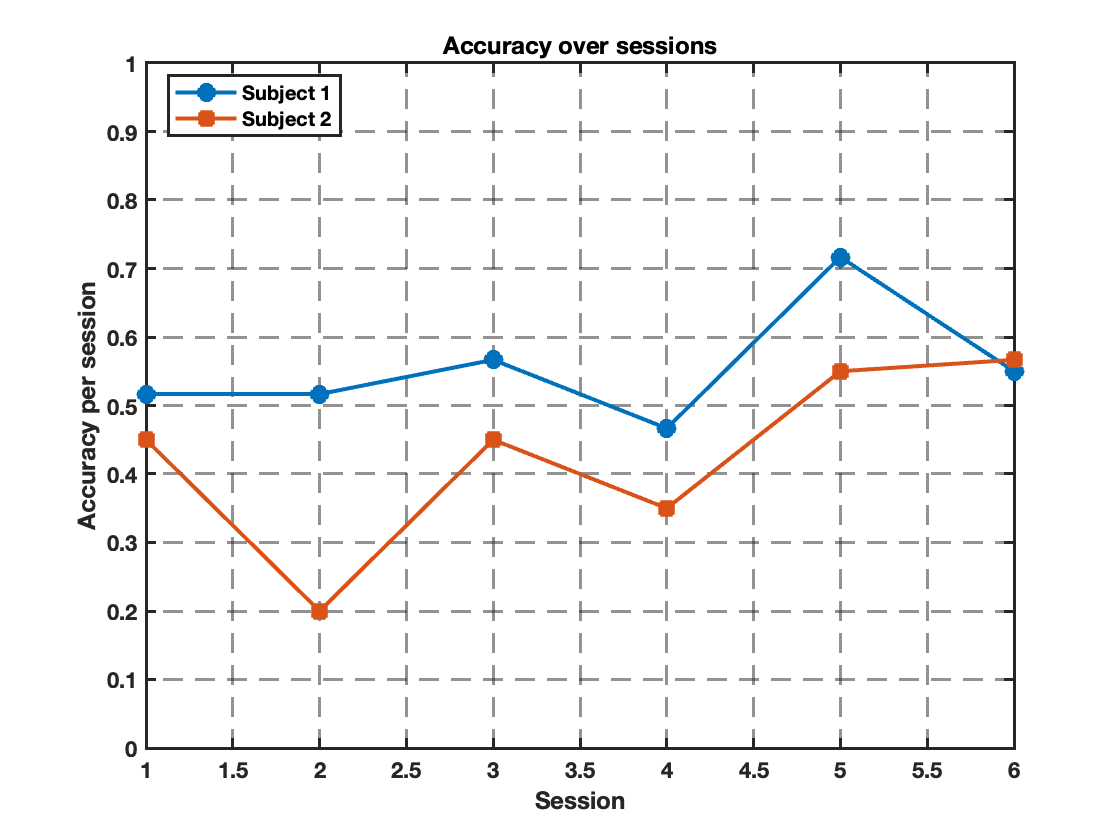
\includegraphics[width=0.7\textwidth]{1_1.png}
\end{center}

Now, let's do some statistical analysis on the command delivery accuracy and timeout percentages over sessions. We will attempt to fit a first-degree polynomial to the data. After this, we can compute an $R^2$ value to see how well the data fits the model. We see that the accuracy and timeout percentages are not well fit by a first-degree polynomial. This is because the data is not linearly correlated with the session number. Thus, this is not statistically significant.

\begin{center}
    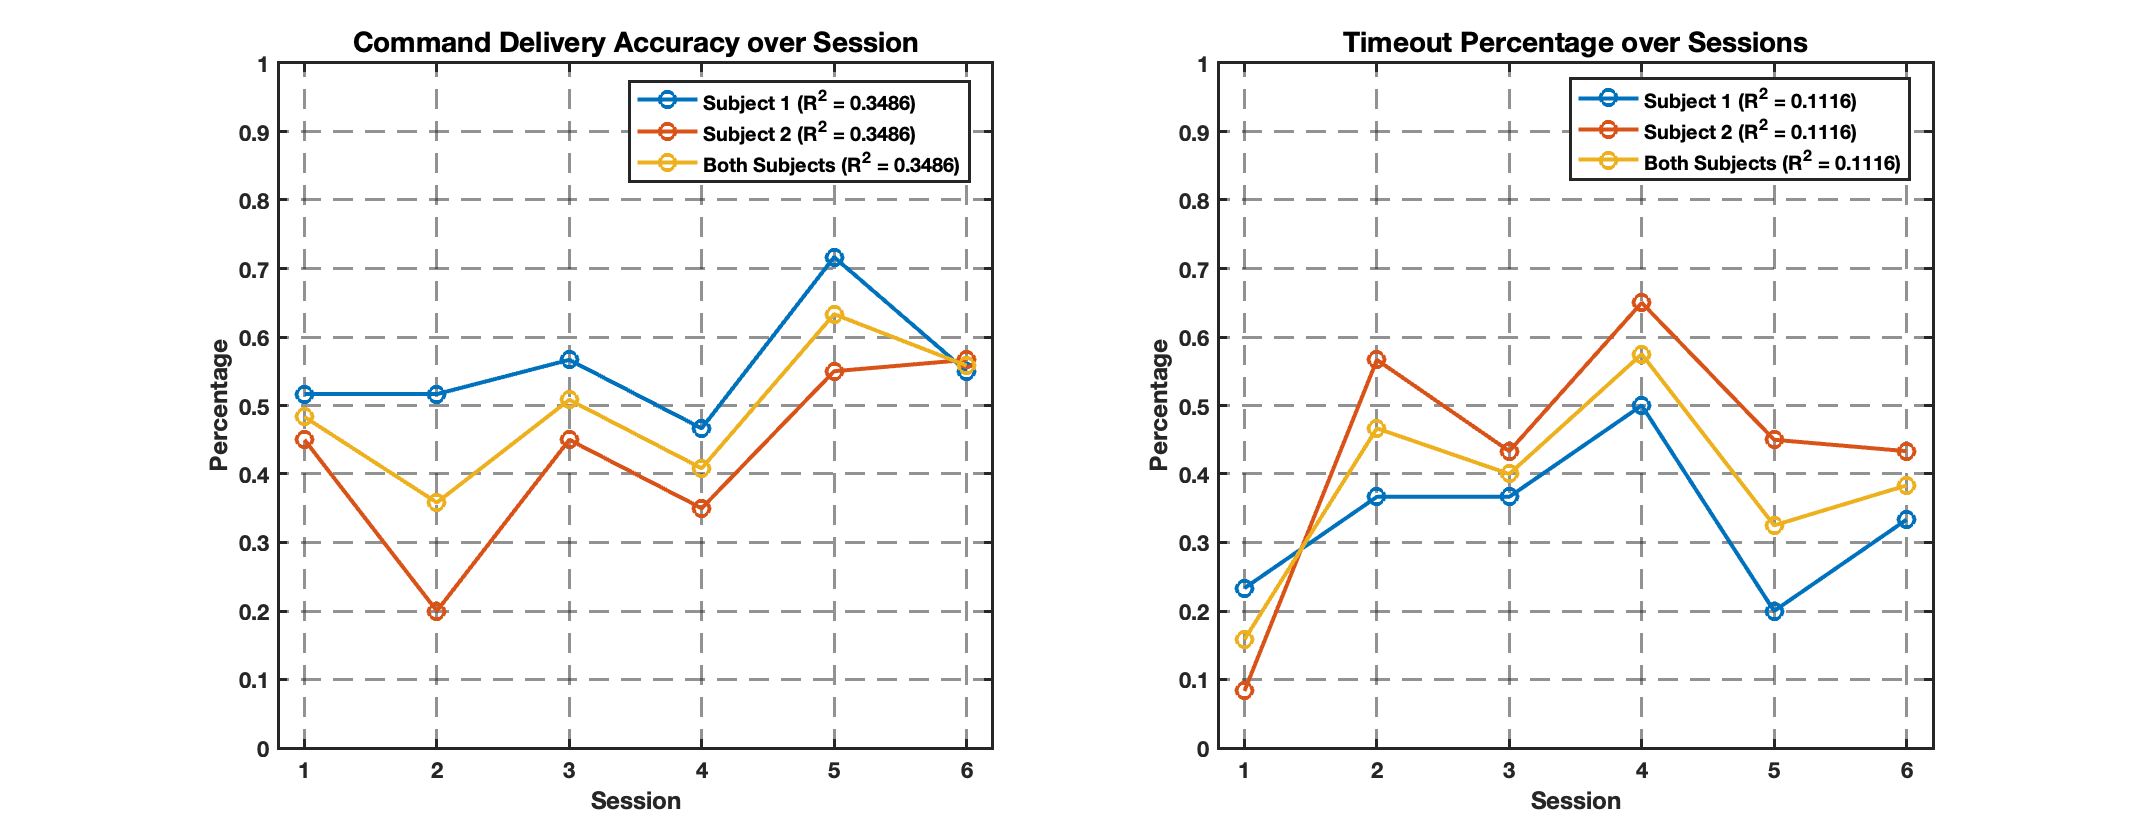
\includegraphics[width=\textwidth]{1_2.png}
\end{center}

Now, we can compare accuracy and timeouts to the first session. We will use a t-test to compare each session against the first one. We find that generally the p-values are high for the command delivery accuracies and low for the timeout percentages, though not all of them are statistically significant. It appears that after session 3, subject 2's p-values drop significantly which may be a session at which statistical significance emerges.

\begin{center}
    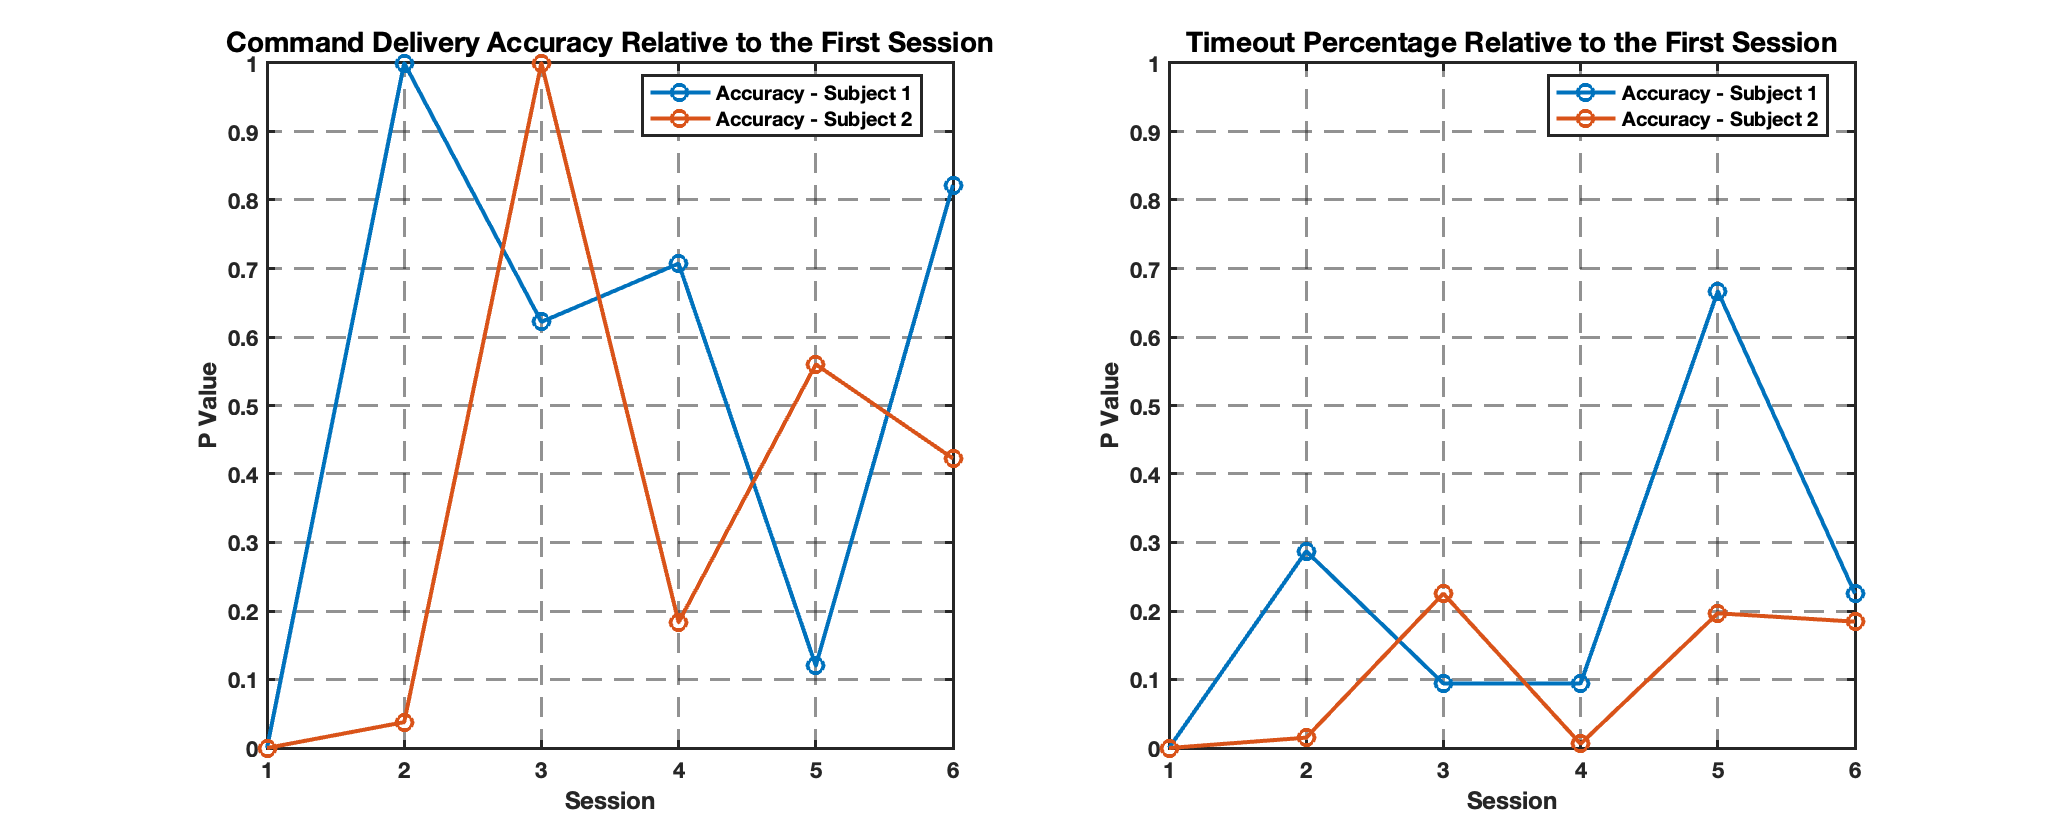
\includegraphics[width=\textwidth]{1_3.png}
\end{center}

\section{Discriminability of Features}
To discriminate features, we will start by using \texttt{pwelch} to extract PSD features. Then, we can compute Fisher scores from the extracted features for each subject. Below, we can see the top 10 features for subject 2. The features seem relatively unstable across sessions which could result from many factors, such as the subject's attention level, the subject's mental state, or the subject's ability to concentrate.

\begin{center}
    \begin{tabular}{c c l l}
        \toprule
        Rank & Value   & Channel & Band \\
        \midrule
        1    & 0.58934 & C3      & 18   \\
        2    & 0.56516 & P3      & 18   \\
        3    & 0.56313 & F7      & 18   \\
        4    & 0.56102 & T7      & 18   \\
        5    & 0.55893 & M1      & 18   \\
        6    & 0.55837 & P8      & 18   \\
        7    & 0.55472 & P4      & 18   \\
        8    & 0.55434 & CP5     & 18   \\
        9    & 0.55335 & F8      & 18   \\
        10   & 0.55265 & P7      & 18   \\
        \bottomrule
    \end{tabular}
\end{center}
$$\textnormal{Table 1: Top 10 Features for Subject 2}$$

Now, we can sum the Fisher scores for all the bands per EEG channel and show the topoplots per subject across sessions. It seems that the topoplots are relatively unstable across sessions which may make it hard to discriminate features. This may be due to the previous feature extraction and may indicate that we are just analyzing noise. This also makes it hard to draw conclusions about the physiological relevance of the features.

\begin{center}
    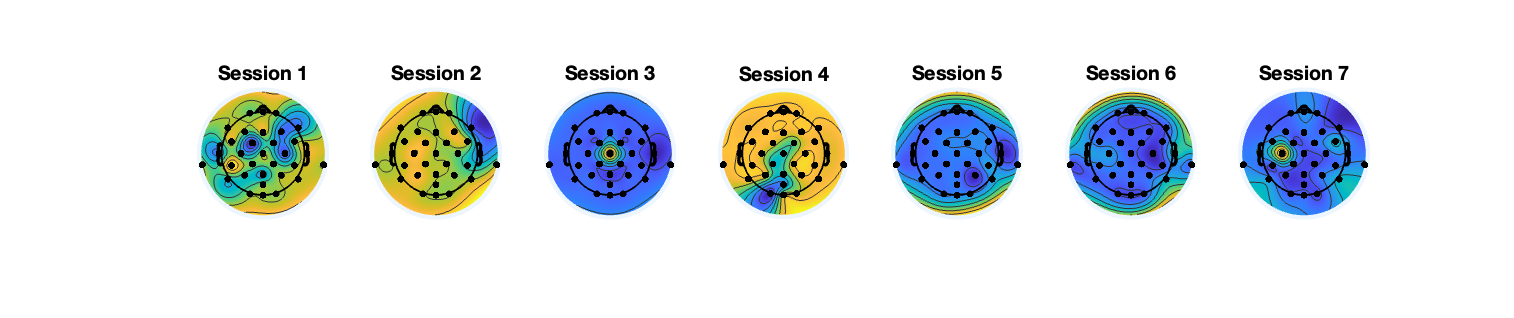
\includegraphics[width=\textwidth]{subj1_topo.png}
\end{center}
$$\textnormal{Figure 1: Topoplots for Subject 1}$$

\begin{center}
    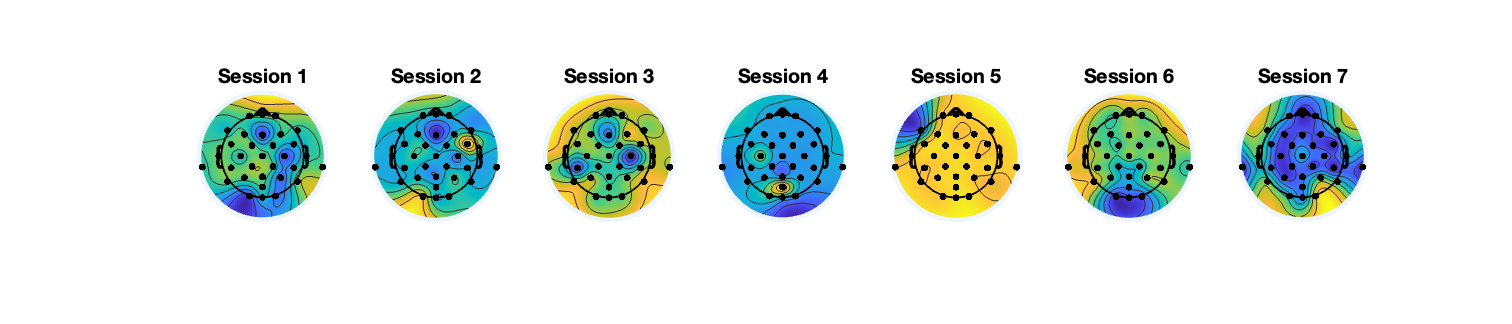
\includegraphics[width=\textwidth]{subj2_topo.png}
\end{center}
$$\textnormal{Figure 2: Topoplots for Subject 2}$$

Finally we will take the channel and band feature with the highest Fisher score on the last online session and track it across all sessions. We can see that for both subjects we don't have a strong correlation, though subject 2 has a significantly stronger correlation than subject 1. This may be due to the data quality of errors during feature extraction.

\begin{center}
    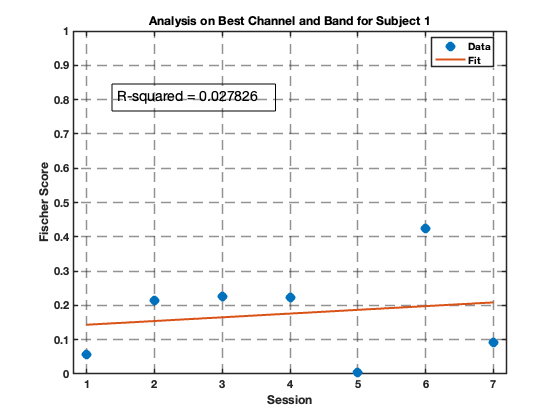
\includegraphics[width=0.7\textwidth]{2_4.png}
\end{center}

\begin{center}
    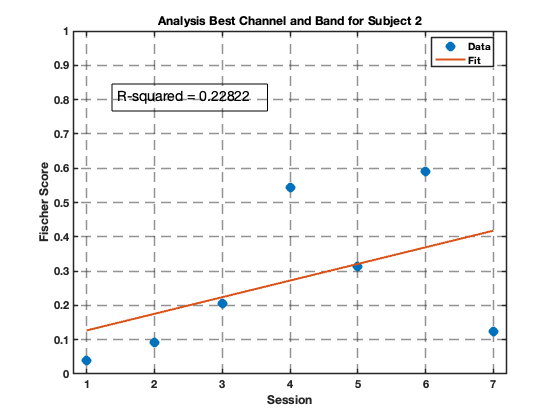
\includegraphics[width=0.7\textwidth]{2_5.png}
\end{center}

We can also look at the top 10 features for subject 2 and correlate the discriminability of these features across sessions to the average command delivery accuracy. This has a much better correlation which may indicate that the features we found are relevant to the task at hand.

\begin{center}
    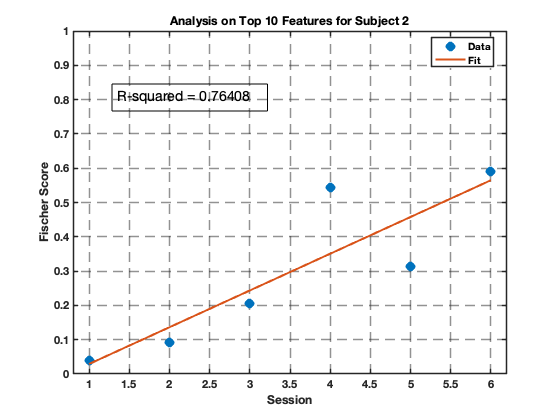
\includegraphics[width=0.7\textwidth]{2_6.png}
\end{center}

\end{document}